\texttt{minimum\_walk([0, 2, 3, 1], 0)}

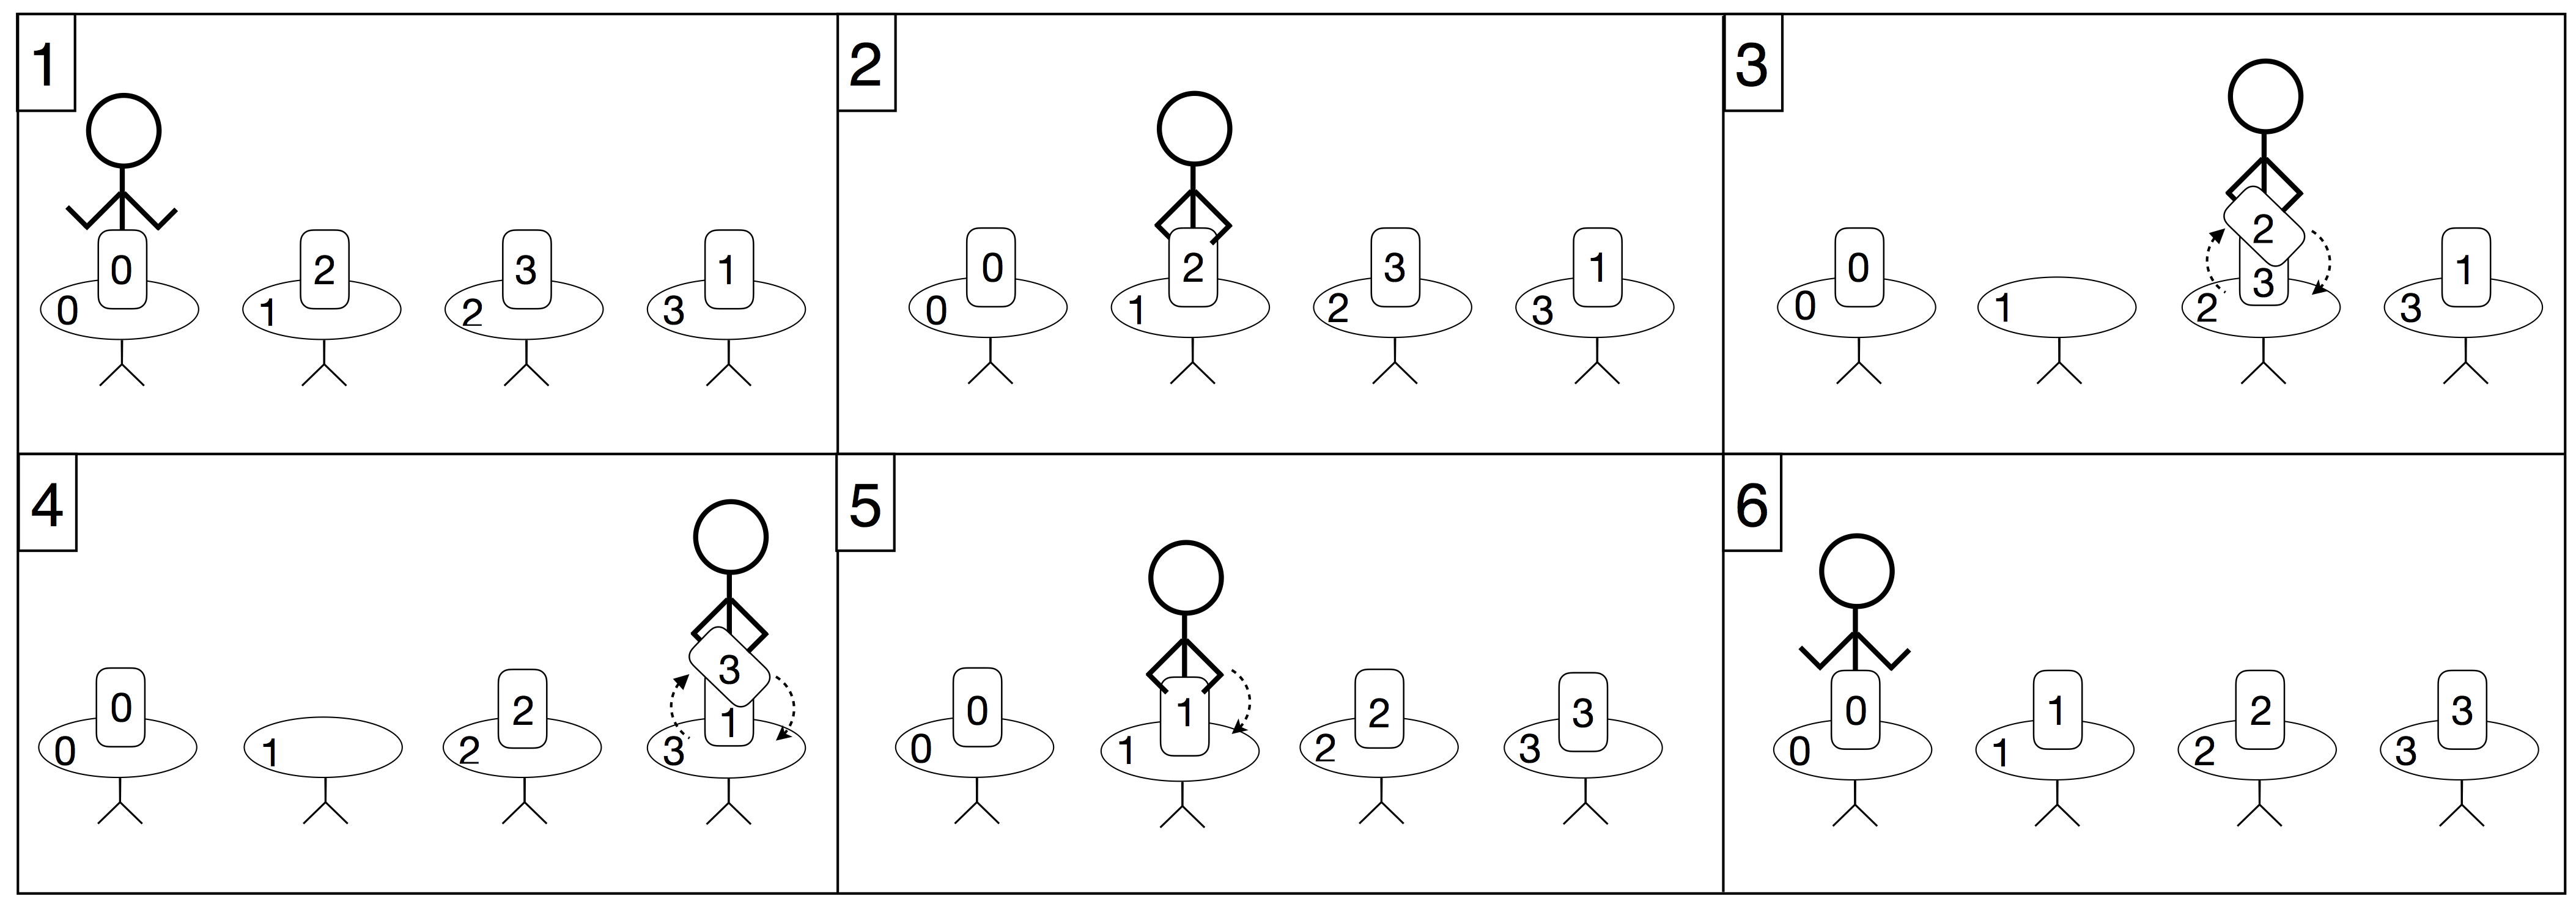
\includegraphics[scale=0.5]{books.png}

In this example, $n=4$ and Aryan is at table $0$ at the beginning.
He sorts the books as follows:
\begin{itemize}
\item He walks to table $1$ and picks up the book lying on it. This book should be put on table $2$.
\item Then, he walks to table $2$ and switches the book he is carrying with the book on the table.
The new book he is carrying should be put on table $3$.
\item Then, he walks to table $3$ and switches the book he is carrying with the book on the table.
The new book he is carrying should be put on table $1$.
\item Then, he walks to table $1$ and puts the book he is carrying on the table.
\item Finally, he walks back to table $0$.
\end{itemize}

Note that book on table $0$ is already in the correct place, table $0$, so Aryan does not have to pick it up.
The total distance he walks in this solution is $6$ meters.
This is the optimal solution; hence, the procedure should return $6$.